\begin{figure}
	\centering
	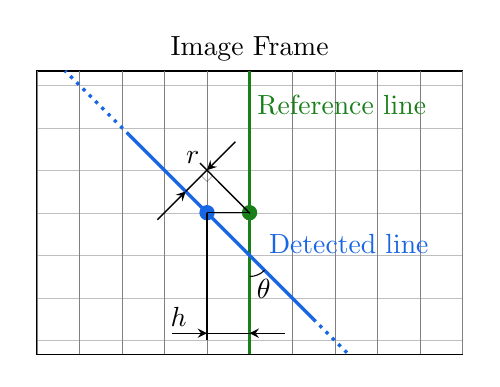
\begin{tikzpicture}[x=0.018cm,y=0.018cm]
\definecolor{my_green}{rgb}{0.1, 0.5, 0.1}
\definecolor{my_blue}{rgb}{0.1, 0.4, 0.9}


% Rectangle
\node (rect) at (0, 0) [draw, minimum width=5.4cm, minimum height=3.6cm] {};
\draw [] (rect) node[above, yshift=1.8cm] {Image Frame};
\foreach \i in {-5 ,...,5} {
        \draw [line width=0.05,gray] (\i * 30, -100) -- (\i * 30,100)  node [below] at (\i * 30,100) {};
        }

\foreach \i in {-3 ,...,3} {
    \draw [line width=0.05,gray, opacity=0.5] (-150, \i * 30) -- (150, \i * 30)  node [below] at (150, \i * 30) {};}
% Green middle line
\draw [color=my_green, line width=1.2] (0, -100) -- (0, 100) ;

% Blue middle line
\draw [color=my_blue, line width=1.2][fill={rgb, 255:red, 65; green, 117; blue, 5 }  ,fill opacity=1 ]   (100 - 5*11, -100 + 5 * 11 - 30) -- (-100 + 5*3, 100 - 5 * 3 - 30) ;

%  Center circles
\draw [color=my_green, fill=my_green](0, 0) circle (5) ;
\draw [color=my_blue, fill=my_blue] (-30, -0) circle (5) ;

% Blue dashed line
\draw [dotted][color=my_blue, line width=1.2] (100 - 5 * 11, -100 + 5 * 11  - 30) -- (70, -100) ;

\draw [dotted][color=my_blue, line width=1.2](-100 + 5*3, 100 - 5*3 - 30) -- (-130, 100) ;

% Connect two center circles
\draw [line width=0.5](0.25, -0.5) -- (-35, 35) ;

% Connect two center points
\draw [line width=0.5](-30, -0) -- (0, 0);

% Draw arrows
\draw [line width=0.5][stealth-](-30, 30) -- (-30 + 20,  30 + 20);
\draw [line width=0.5][stealth-](-45, 15) -- (-45 - 20, 15 - 20);

% Connect two arrows
\draw [line width=0.5](-30, 30) -- (-45, 15);
% Perpendicular symbol
\draw [line width=0.1](-30 + 4, 30 - 4) -- (-30, 30 - 8);
\draw [line width=0.1](-30 - 4, 30 - 4) -- (-30, 30 - 8);

% Draw vertical line
\draw [line width=0.5](-30, 0) -- (-30, -10 - 80);
\draw [line width=0.5][stealth-](0, -10 - 80  +5 ) -- (0 + 25, - 10 - 80 + 5); 
\draw [line width=0.5][stealth-](-30, -10-80  +5 ) -- (-30 - 25, -10-80 + 5); 
\draw [line width=0.5](-30, -10-80 + 5) -- (0, -10-80 + 5);

%Draw angle arc
\draw (0,-45) arc (270:315:15);

% Draw texts
\draw [color=my_green] (65, 90) node[below] {Reference line};
\draw [color=my_blue] (70, -8) node[below] {Detected line};
\draw (-40, 50) node[below] {$r$};
\draw (-50, -60) node[below] {$h$};
\draw (10, -40) node[below] {$\theta$};




\end{tikzpicture}
	\vspace{0.5ex}
	\caption{Illustration of a reference and detected line onto the image frame.}
	\vspace{-1.5ex}
	\label{fig:lineeval}
\end{figure}